\section[Limits on $t\bar{t}H$ production]{Limits on \boldmath{$t\bar{t}H$} production}

For the single-lepton search the best-fit signal strength is $\mu=1.6\pm1.1$. Since no significant excess of events above the background expectation is found for the SM Higgs boson with mass of 125 GeV, a $95\%$ CL upper limit on the signal strength modifier is set. A signal cross section larger than 3.6 times the SM prediction is excluded at $95\%$ CL. The expected exclusion is 2.2 times the SM prediction in the absence of the $t\bar{t}H$ process.\par
Combining those results with the dilepton search, the expected sensitivity improves by $15\%$ with respect to the single-lepton-only search.
The best-fit $\mu$ values for the single-lepton and dilepton searches, and their combination, are shown in figure \ref{sec:ttH:fig:musum}.
\begin{figure}[h!]
 \centering
 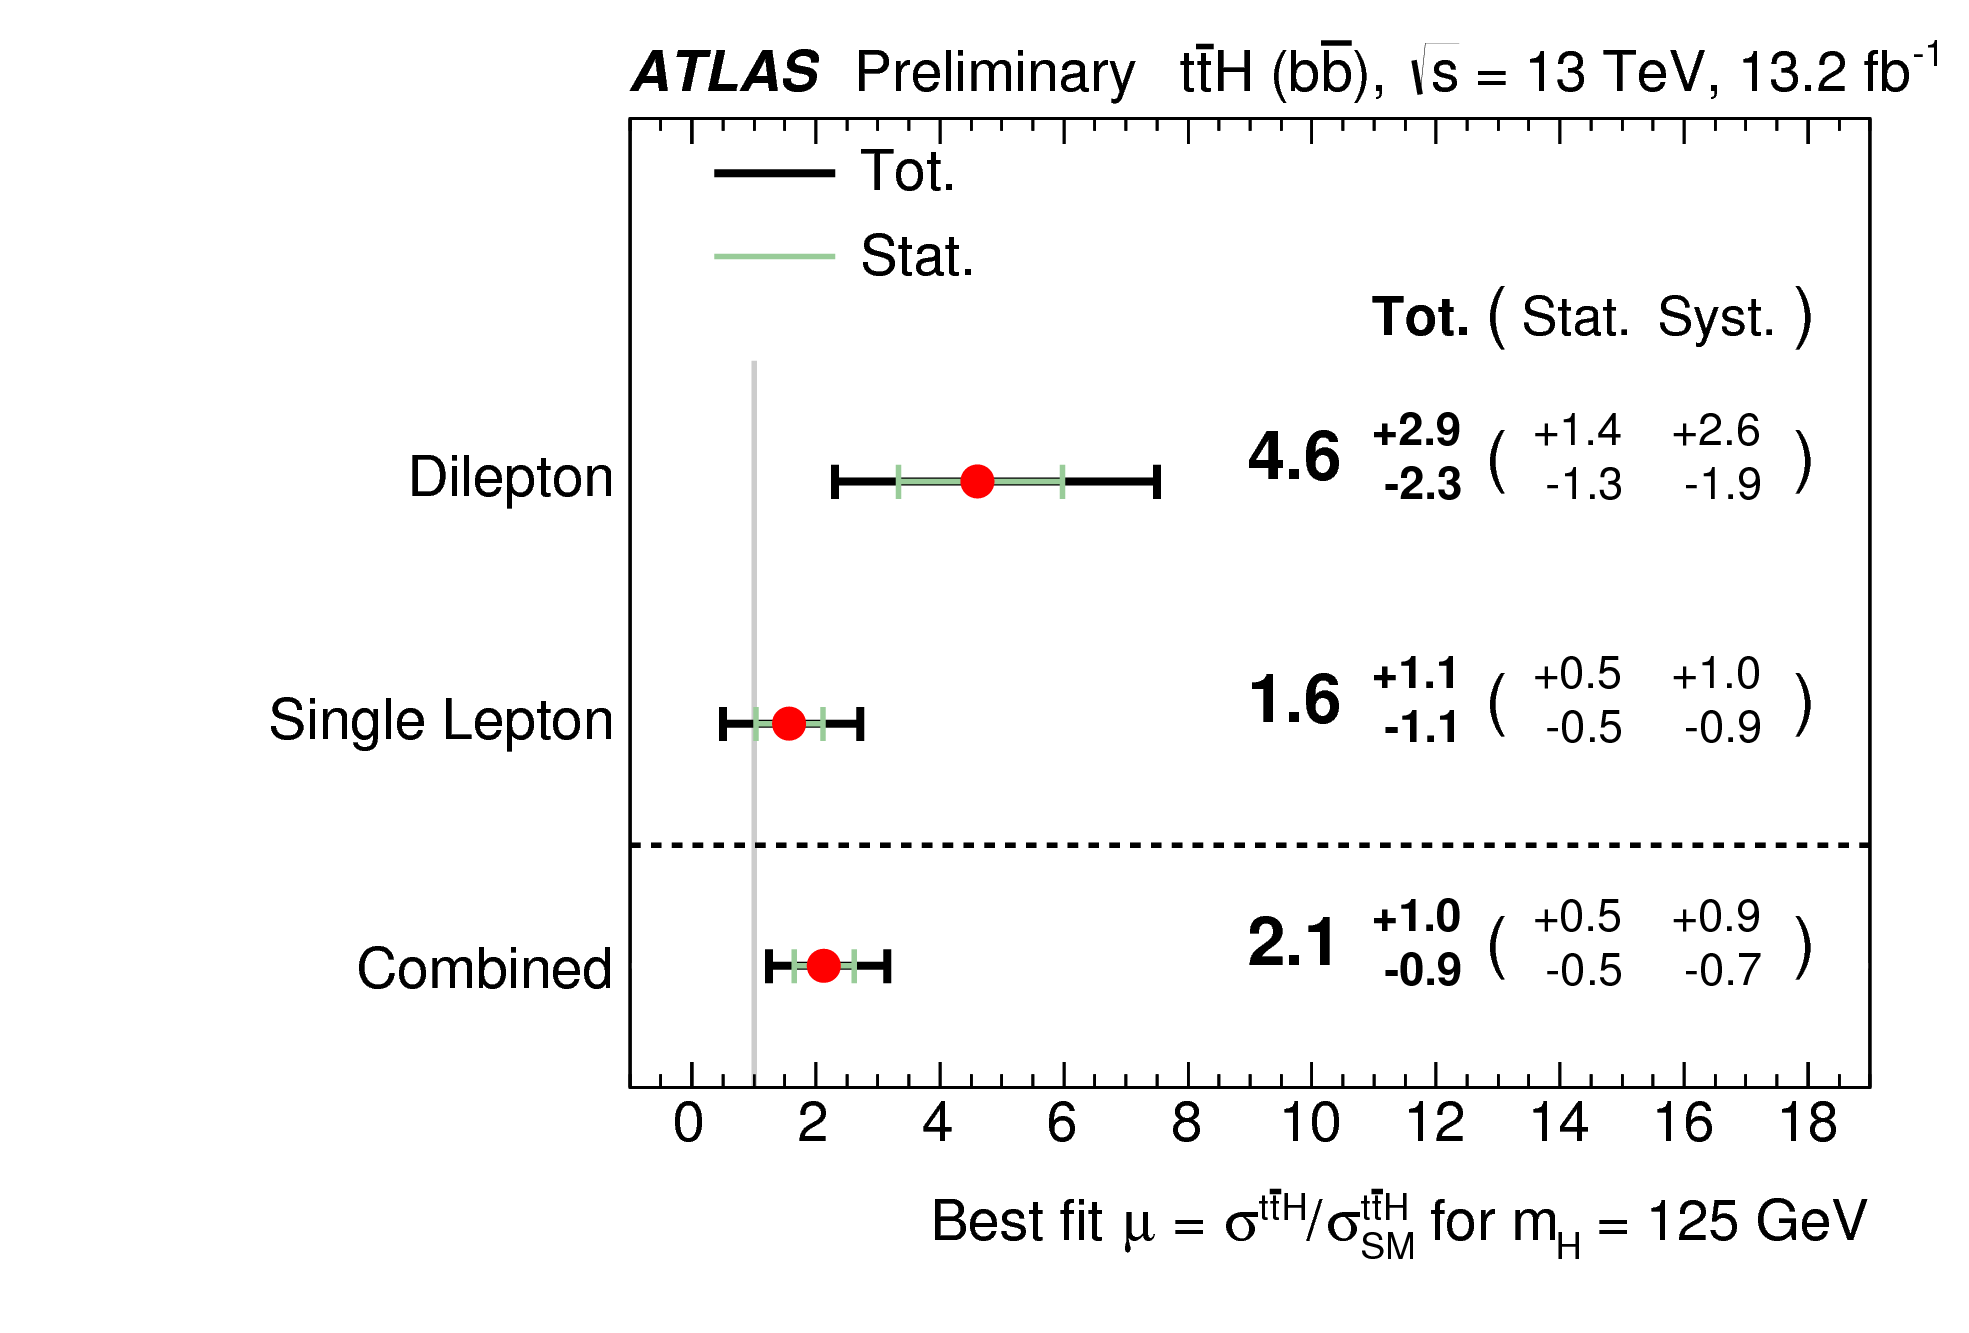
\includegraphics[width=0.7\textwidth]{figures/ttH/fig_13.png}
\captionsetup{width=0.85\textwidth}  \caption{\small Signal-strength measurements for the individual channels, as well as their combination.}
\label{sec:ttH:fig:musum}
\end{figure}
The fitted signal strength for the combined analysis is $\mu = 2.1^{+1.0}_{-0.9}$. The observed (expected) significance of the signal is 2.4 (1.2) standard deviations. The observed and expected limits for both searches and their combination are shown in figure \ref{sec:ttH:fig:limitsum}. A signal cross section 4.0 times larger than predicted by the SM is excluded at $95\%$ CL. The expected exclusion is 1.9 times the SM prediction in the absence of the $t\bar{t}H$ process, and 2.7 times the SM prediction if the $t\bar{t}H$ process is present with the SM predicted rate.\par
Finally, figure \ref{sec:ttH:fig:sbbinssum} summarises the post-fit event yields as a function of $\log_{10}(S/B)$, for all bins of the distributions used in the combined fit of the single-lepton and dilepton channels. The signal is normalised to the fitted value of the signal strength ($\mu = 2.1$) and a signal 4.0 times larger than predicted by the SM, which is excluded at $95\%$ CL, is also shown.

\begin{figure}[h!]
\centering
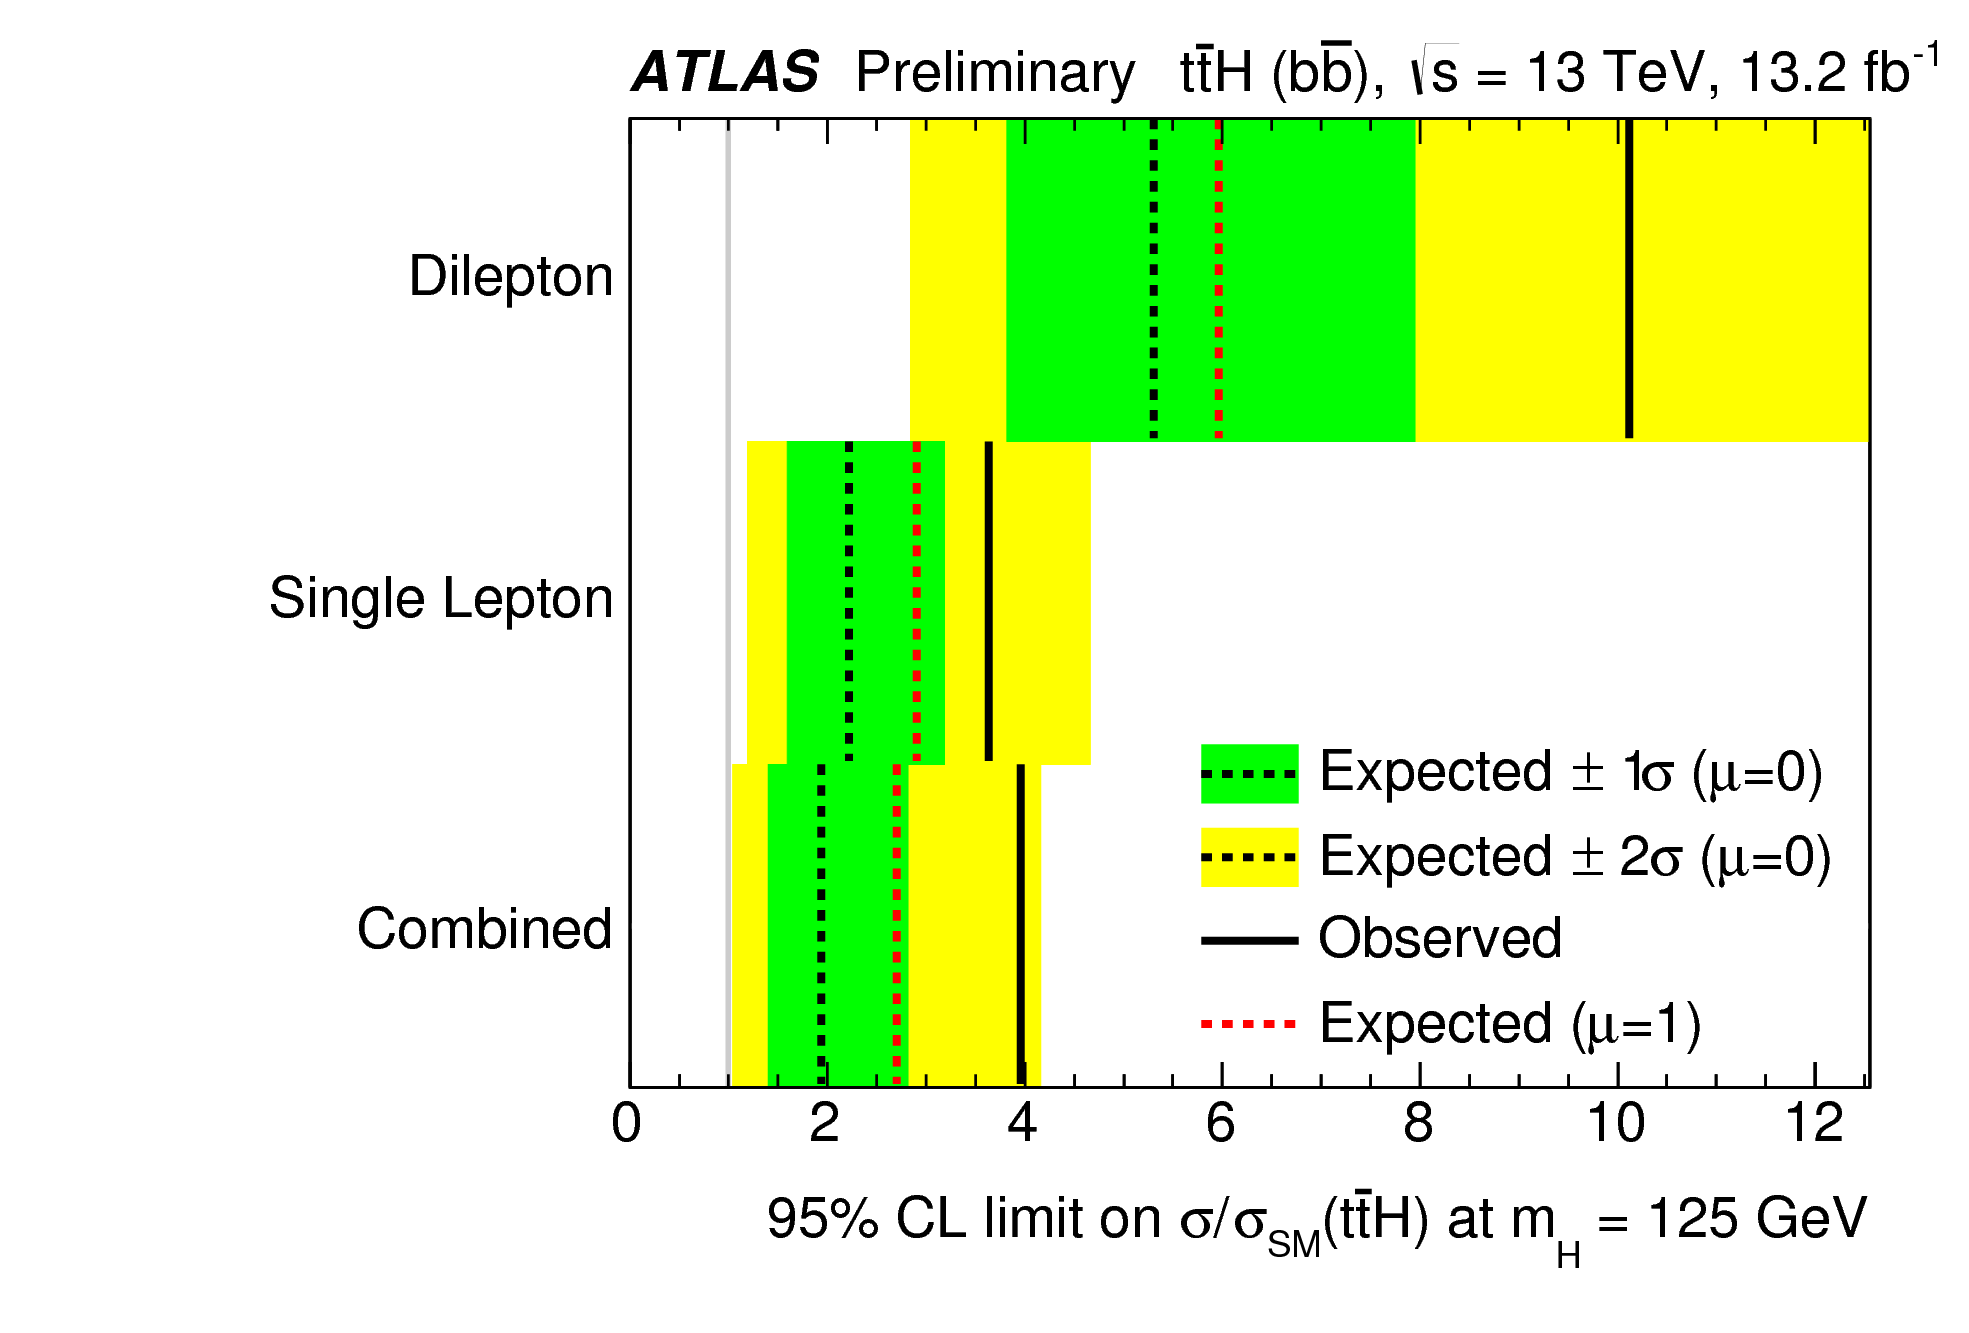
\includegraphics[width=0.7\textwidth]{figures/ttH/fig_14.png}
\captionsetup{width=0.85\textwidth}  \caption{\small Summary of the $95\%$ CL upper limits on $\sigma(t\bar{t}H)$ relative to the SM prediction for the individual channels, as well as their combination.}
\label{sec:ttH:fig:limitsum}

\centering
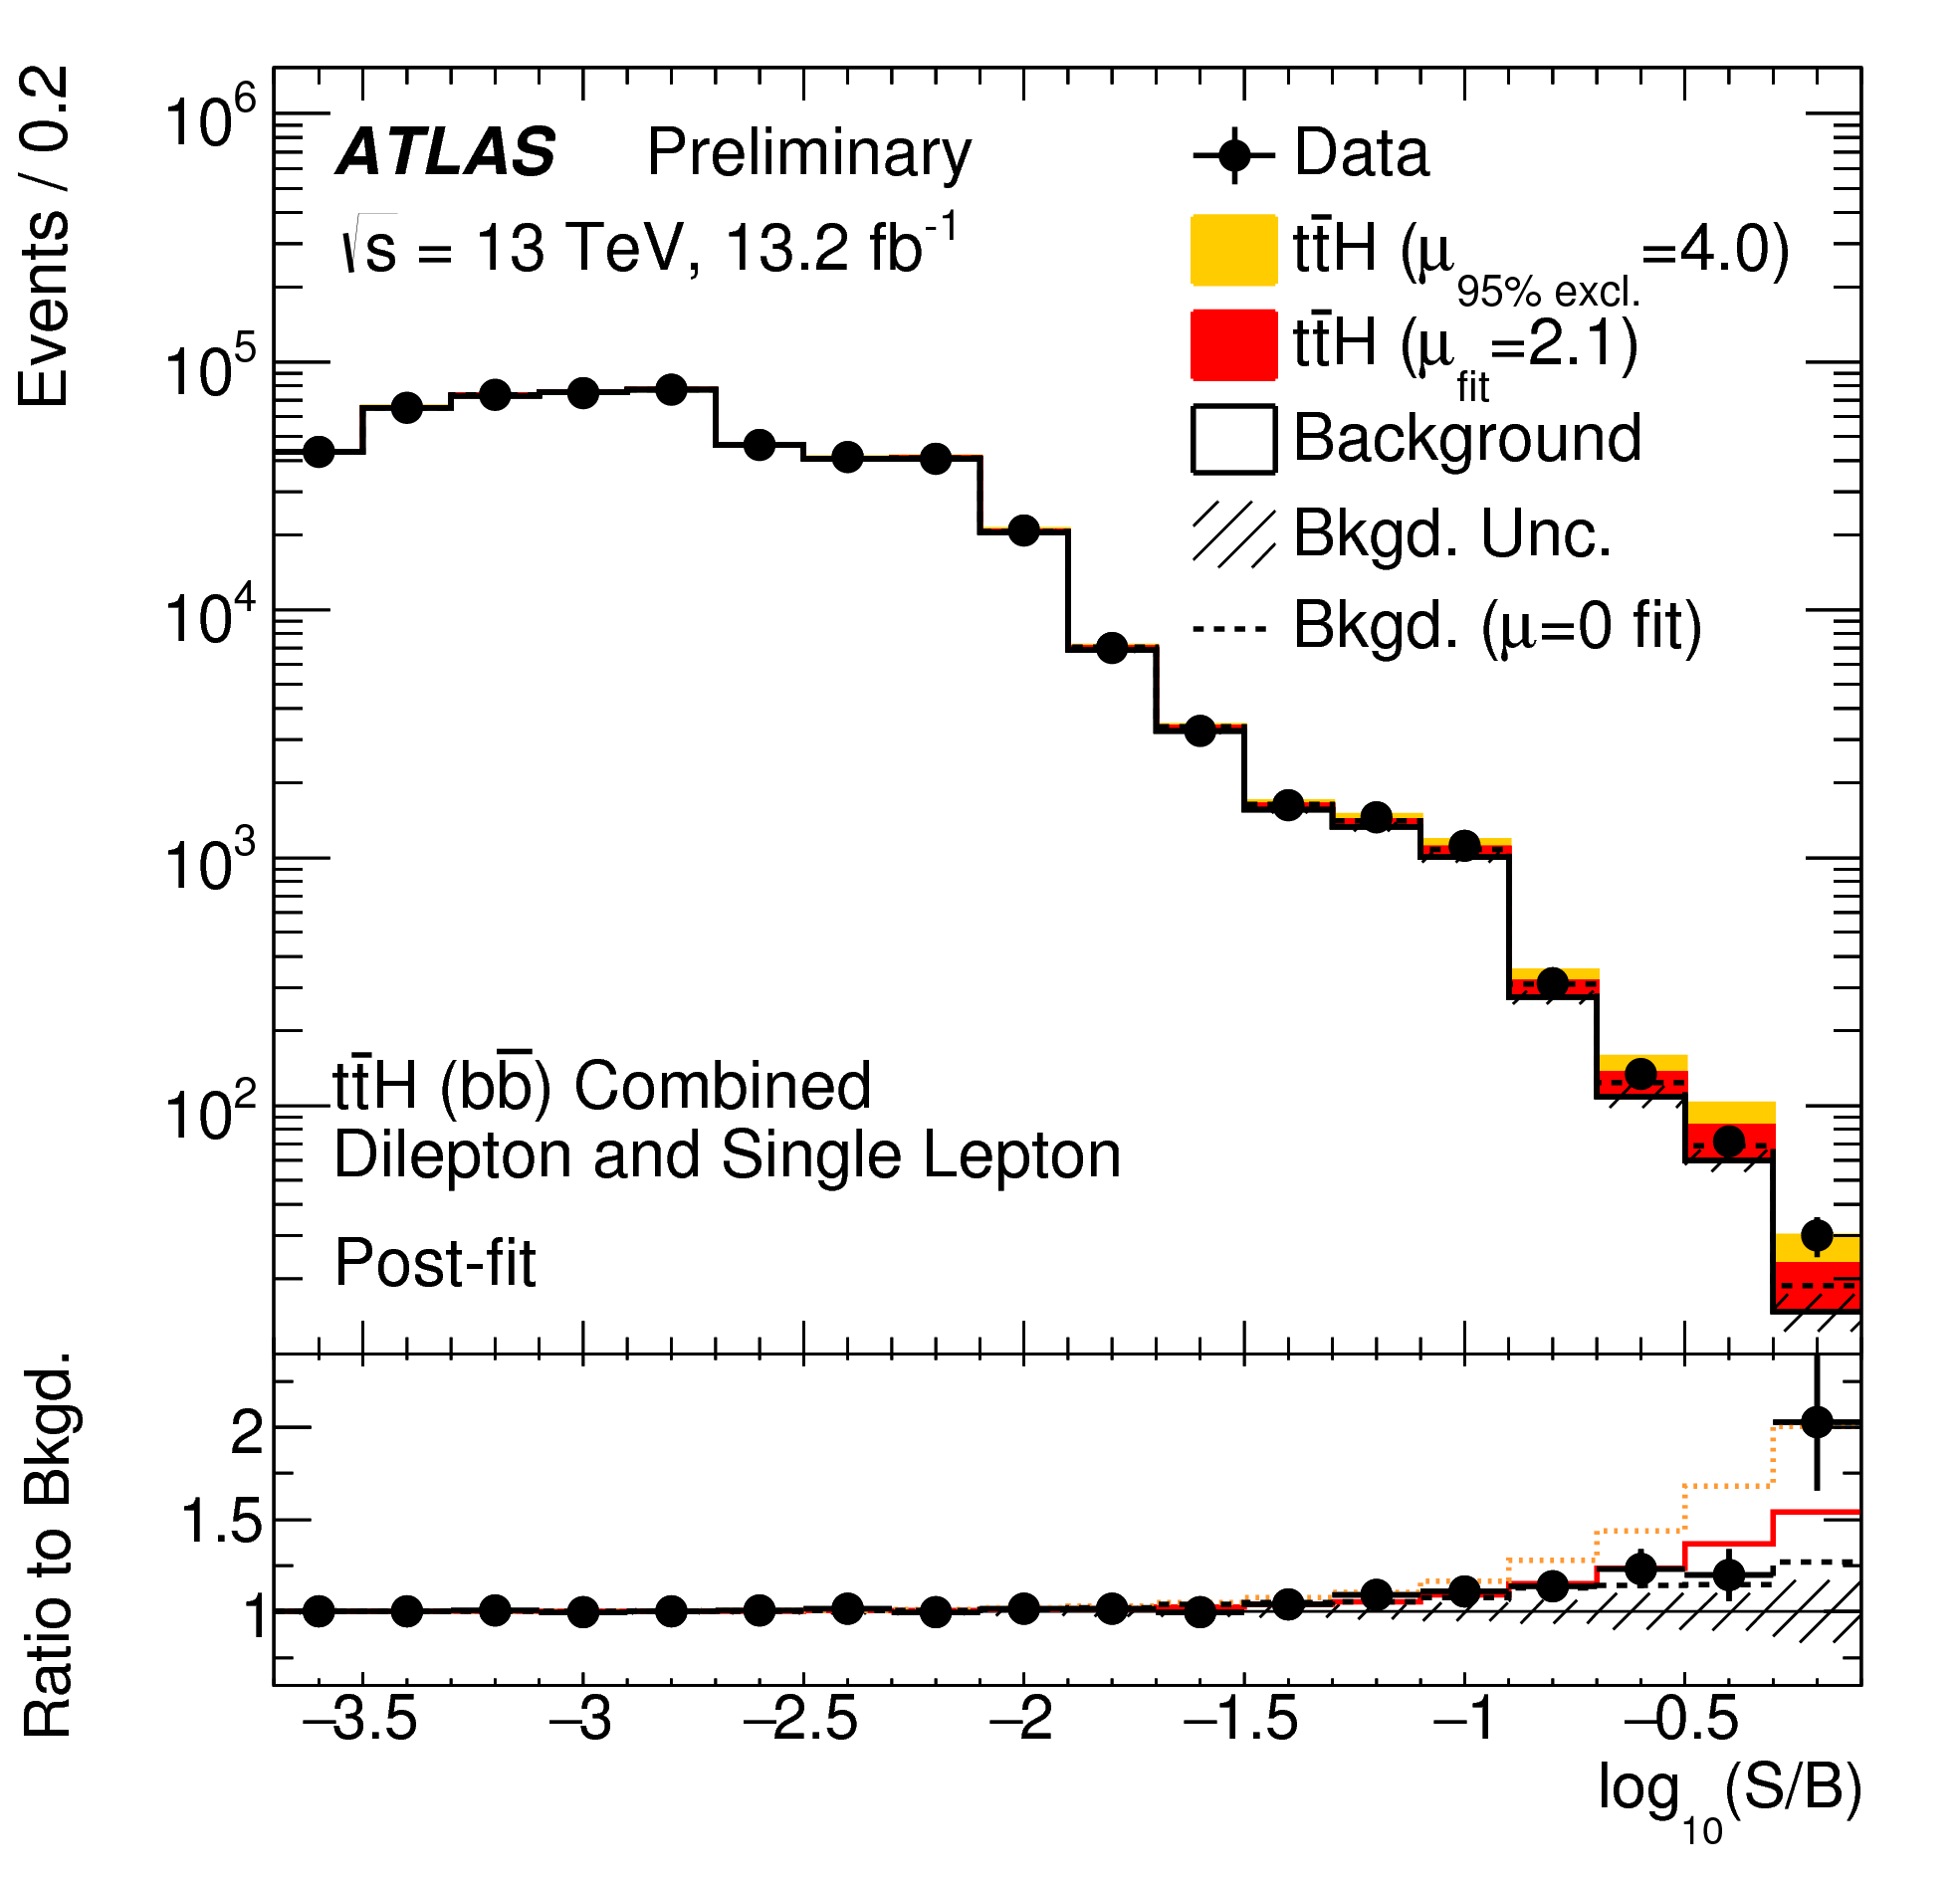
\includegraphics[width=0.5\textwidth]{figures/ttH/fig_12.png}
\captionsetup{width=0.85\textwidth}  \caption{\small Post-fit event yields, as a function of $\log_{10}(S/B)$, where $S$ ($B$) denotes the signal (background) yield, for all bins used in the
combined fit of the single-lepton and dilepton channels. The signal is shown normalised to the best-fit value and to the excluded value. The background is also shown after the fit to data assuming zero signal contribution.}
\label{sec:ttH:fig:sbbinssum}
\end{figure}

\subsection{Comparison with other analyses}

Searches for the $t\bar{t}H$ process have also been performed in ATLAS in the diphoton \cite{ATLAS-CONF-2016-067} and multilepton \cite{ATLAS-CONF-2016-058} final states. The expected exclusion limits are 2.7 and 2.3 times the SM prediction, respectively. The combination \cite{ATLAS-CONF-2016-068} of the three analyses: $b\bar{b}$, diphoton and multilepton, has been performed in order to achieve the most sensitive result.
The best-fit value of the signal strength is $\mu=1.8\pm0.7$. A signal 1.2 times larger than the SM Higgs boson is expected to be excluded in the case of no SM Higgs boson, while a signal 3.0 times  larger than predicted by the SM is excluded at $95\%$ CL. The sensitivity of this combination already exceeds the Run 1 ATLAS combination \cite{Aad:2016zqi}. The fitted signal strengths and $95\%$ CL upper limits are summarised in figures \ref{sec:ttH:fig:combimu} and \ref{sec:ttH:fig:combilimit} respectively, for the individual searches and their combination. The observed (expected) significance is 2.8 (1.8) standard deviations, which represents an improvement of $50\%$ relative to the most-sensitive individual analysis.

\begin{figure}[p!]
  \centering
  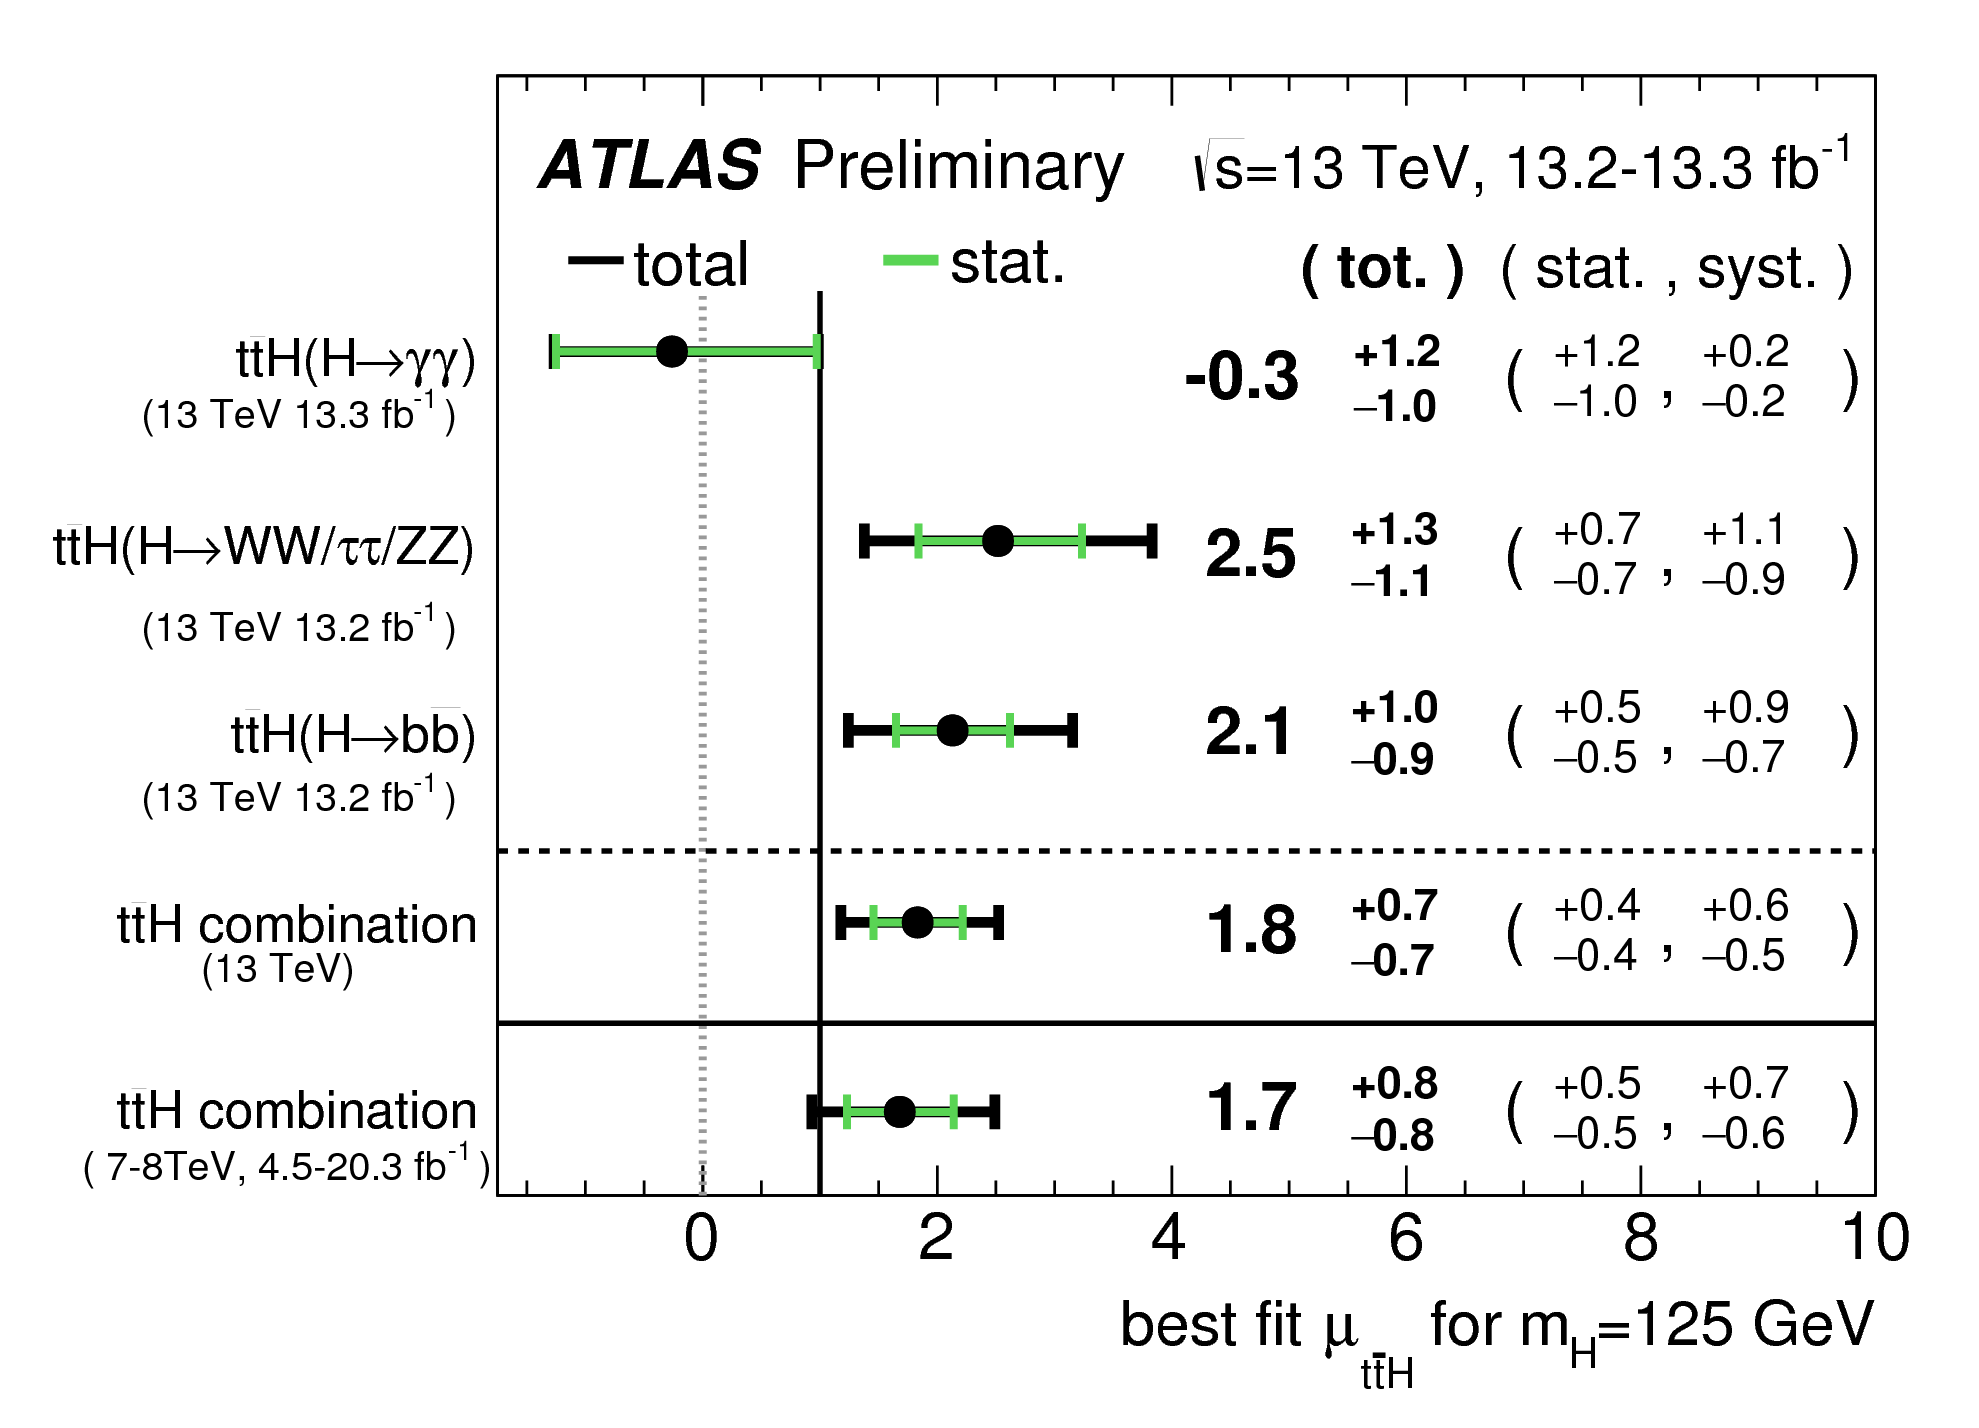
\includegraphics[width=0.7\textwidth]{figures/ttH/fig_01.png}
 \captionsetup{width=0.85\textwidth}  \caption{\small Signal-strength measurements in the individual channels and for the combination.}
  \label{sec:ttH:fig:combimu}

  \centering
  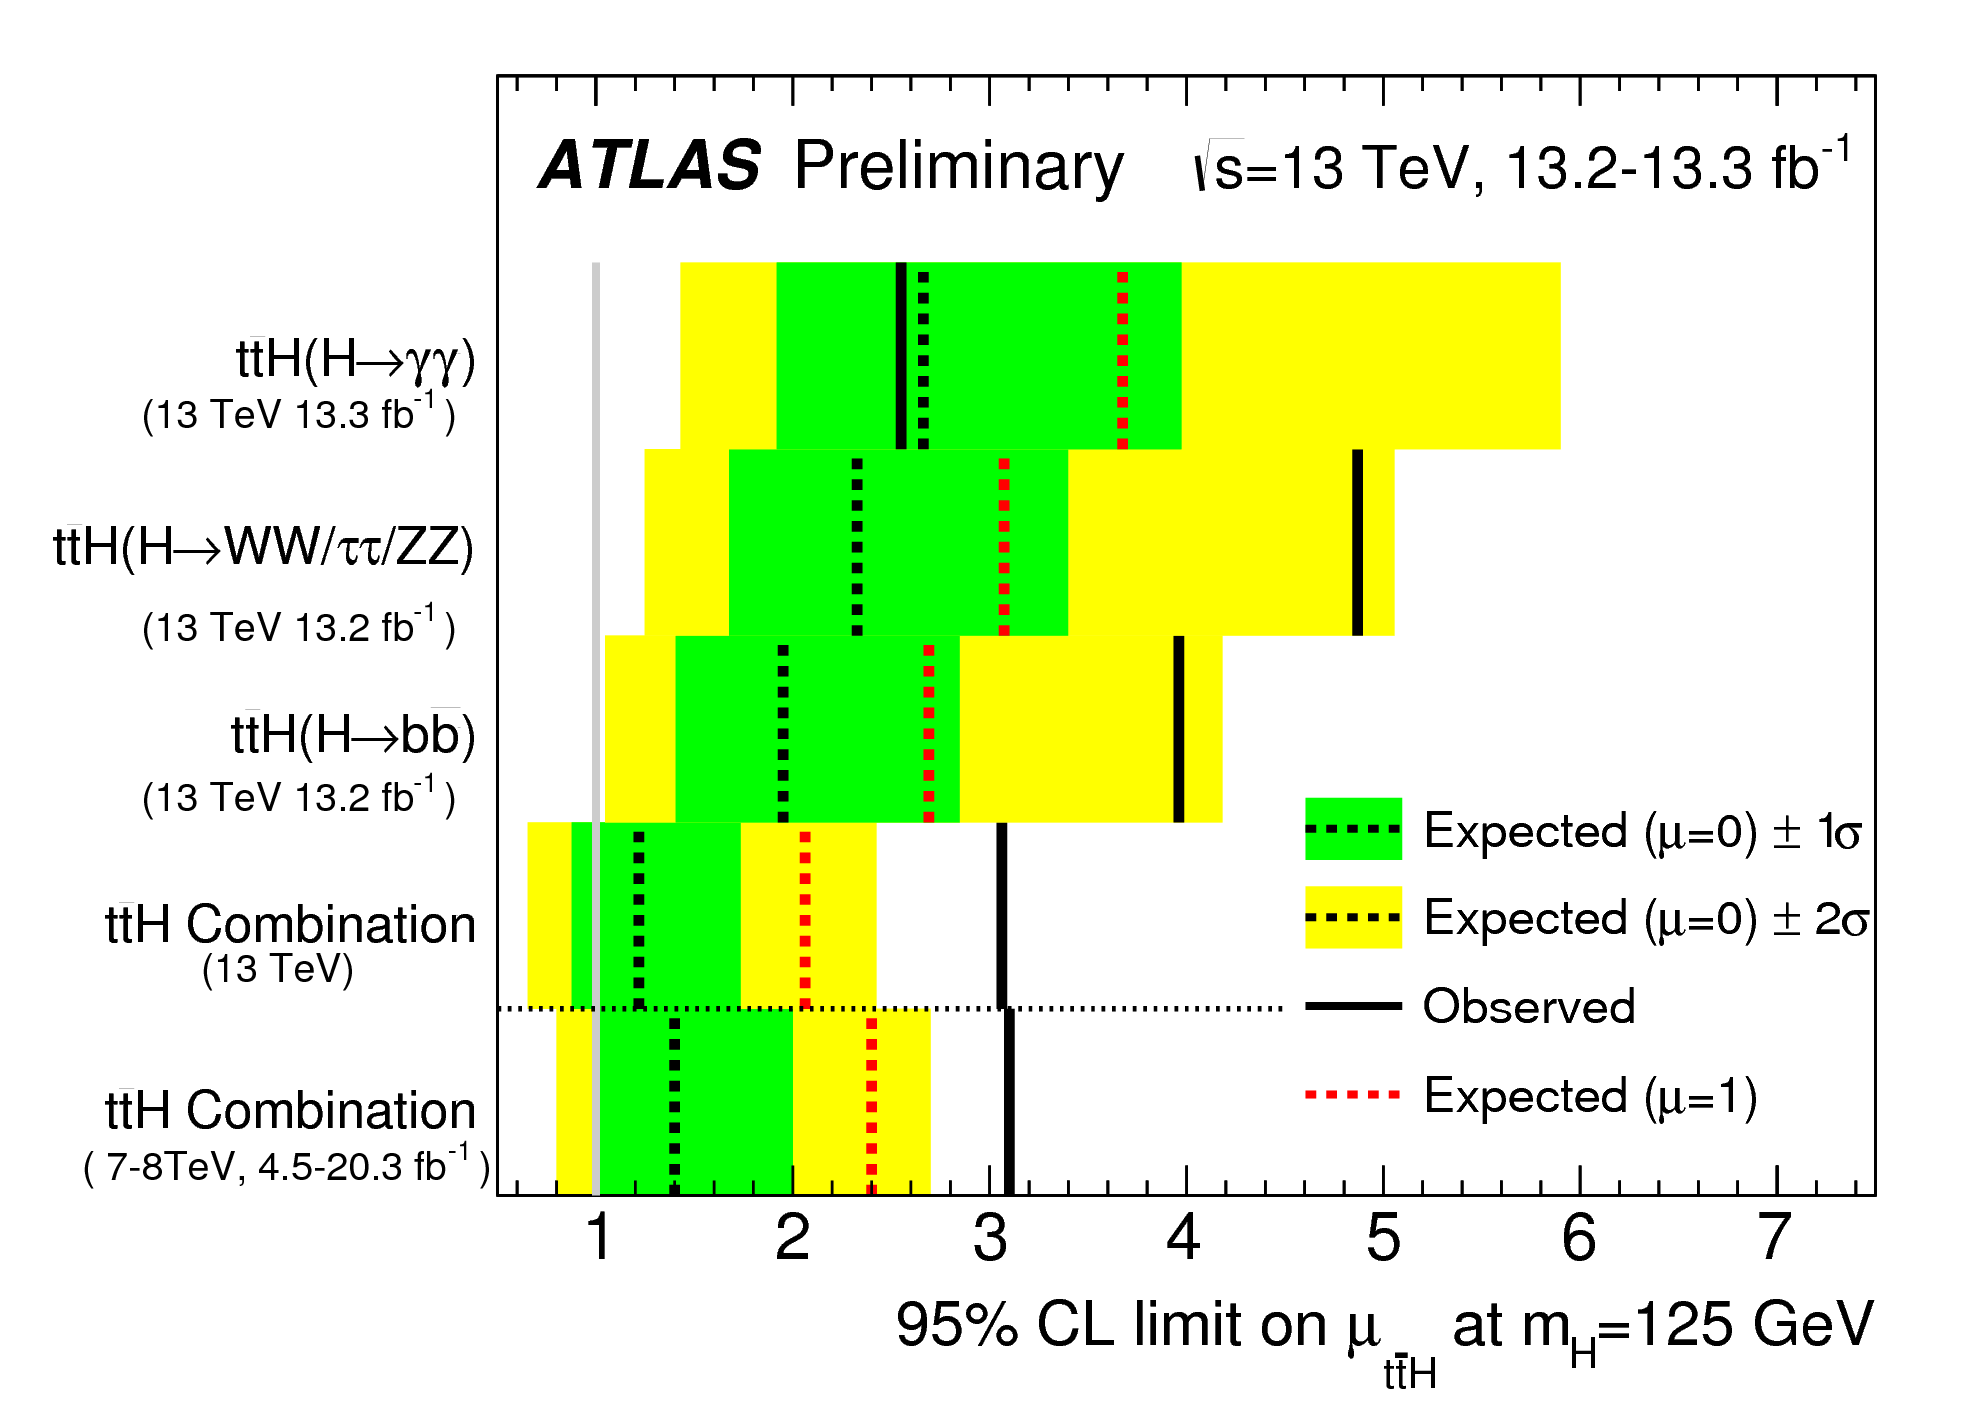
\includegraphics[width=0.7\textwidth]{figures/ttH/fig_03.png}
  \captionsetup{width=0.85\textwidth}  \caption{\small Summary of the of $95\%$ CL upper limits on $\sigma(t\bar{t}H)$ relative to the SM prediction.}
  \label{sec:ttH:fig:combilimit}
\end{figure}




Searches for $t\bar{t}H$ production at $\sqrt{s}=13$ $\tev$ considering several Higgs-boson decay modes (including $H \to b\bar{b}$) have been published by the CMS Collaboration \cite{CMS-PAS-HIG-16-022,CMS-PAS-HIG-16-038,CMS-PAS-HIG-16-020}. The search in the $H \to b\bar{b}$ channel uses 12.9 fb$^{-1}$ of data, and as final discriminating variable it uses the matrix-element method in conjunction with a classification BDT. The observed (expected) $95\%$ CL upper limit on $\sigma(t\bar{t}H)$ is 1.5 (1.7) times the SM prediction. The fitted signal strength, combining single-lepton and dilepton channels, is $\mu = -0.2\pm0.8$. The error on $\mu$ is reduced compared to the ATLAS result due to the simplified systematic model used by CMS.\par
In summary, the analysis  for the $t\bar{t}H$ process described in this dissertation is the most sensitive search to date in ATLAS and competitive with that of the CMS Collaboration.